\section{Desenvolvimento}

A implementação do \textit{front end} teve como base o código Java disponibilizado no apêndice A do livro-texto \cite{aho2007compilers}. A seguir serão discutidas as estruturas de dados utilizadas em cada uma das partes da implementação do \textit{front end}, bem como as suas relações com o funcionamento do programa.

\subsection{Analisador Léxico}
A análise léxica do \textit{front end} é implementada através do pacote \texttt{lexer}. O funcionamento geral é baseado na identificação de \textbf{tokens} a partir da entrada. Tais tokens podem ser \textbf{constantes}, \textbf{palavras-chave} (reservadas) ou \textbf{identificadores}. Uma vez identificados, os tokens são passados para o \textbf{parser}, a fim de criar a tabela de símbolos.

\begin{itemize}
\item Classe \textbf{Tag}: é responsável pela definição de constantes para os tokens.
\item Classe \textbf{Word}: é responsável por gerenciar lexemas para identificadores, palavras-chave e \textit{tokens} compostos.
\item Classe \textbf{Real}: é responsável pelos números de ponto flutuante.
\item Classe \textbf{Num}: é responsável pelos números inteiros.
\item Classe \textbf{Token}: é responsável pelas decisões de parse (lexemas ou valores), como pode ser visualizado na figura abaixo.
\item Classe \textbf{Lexer}: implementa função \textit{scan()} para receber os \textit{tokens}.
\end{itemize}

\begin{figure}[H]
	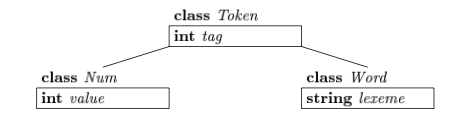
\includegraphics[width=1\textwidth]{imgs/lex_decisions.png}
	\caption{Decisões de parse baseadas na \texttt{tag} da classe \textbf{Token} (lexemas ou valores)}.
	\label{fig:dccnet}
\end{figure}

\subsection{Tabela de Símbolos}
A tabela de símbolos do \textit{front end} é responsável por guardar informações sobre as construções do programa fonte. As entradas da tabela contém informação sobre identificadores (lexema, tipo e posição de armazenamento). 

A tabela de símbolos deve ser capaz de guardar múltiplas declarações do mesmo identificador, cada uma em um escopo diferente. A implementação feita utiliza a noção de escopos para garantir essa premissa.

\begin{figure}[H]
	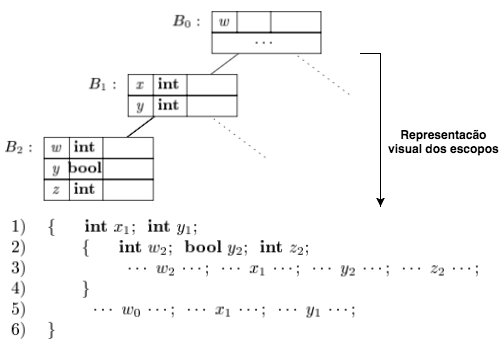
\includegraphics[width=1\textwidth]{imgs/st_scopes.png}
	\caption{Exemplo de blocos de códigos e seus respectivos escopos na tabela de símbolos}.
	\label{fig:dccnet}
\end{figure}

A tabela de símbolos é na verdade uma "cadeia" de tabela de símbolos, cada uma representando seu respectivo escopo. 

A noção de escopos foi implementada através da classe \textbf{Env} presente no pacote \texttt{symbols}. A estrutura de dados utilizada para cada tabela de símbolos foi uma tabela \textbf{hash}. Quando encadeadas, as tabelas de símbolo formam uma estrutura de árvore. A classe \textbf{Env} contém três operações básicas (funções/construtores):

\begin{itemize}
\item \textbf{construtor Env()}: cria nova tabela de símbolos através de uma \textit{Hashtable}. A criação é baseada no escopo corrente, ou seja, se já foi criado algum escopo anterior, o próximo escopo é criado e 'linkado' com o anterior através da variável \texttt{prev}, do tipo \texttt{Env}.
\item \textbf{função put()}: coloca nova entrada na tabela corrente baseada em uma \textbf{chave} (entrada da classe \textbf{Token}) e um \textbf{valor} (entrada da classe \textbf{Id}, do pacote \texttt{iter})
\item \textbf{função get()}: recuperar uma entrada para um identificador, procurando na cadeia de tabelas de símbolos.
\end{itemize}

A seguir é apresentado o trecho de código referente à classe \textbf{Env}:

\begin{lstlisting}[language=Java, caption=Classe Env.java]
public class Env {
    private Hashtable table;
    protected Env prev;

    public Env(Env n) { table = new Hashtable(); prev = n; }

    public void put(Token w, Id i) { table.put(w, i); }

    public Id get(Token w) {
        for( Env e = this; e != null; e = e.prev ) {
            Id found = (Id)(e.table.get(w));
            if( found != null ) return found;
        }
        return null;
    }
}
\end{lstlisting}

\subsection{Analisador Sintático}

A implementação do analisador léxico se faz presente no pacote \texttt{parser}, num arquivo de mesmo nome. A gramática original da linguagem \textbf{SmallL} precisava de adaptações para ser reconhecida por análise descendente(\textit{top-down}). Portanto, os procedimentos implementados na classe \textbf{Parser} são baseados na gramática resultante após a remoção da recursão à esquerda na gramática original.

Se utilizando do fluxo de entrada de tokens, o analisador sintático constrói a árvore de sintaxe com o apoio das funções construtoras do pacote \texttt{inter} e da tabela de símbolos. Um exemplo ilustrativo de árvore de sintaxe pode ser visto na Figura 5, não necessariamente refletindo a gramática da linguagem tratada neste trabalho.

\begin{figure}[H]
	\centering
	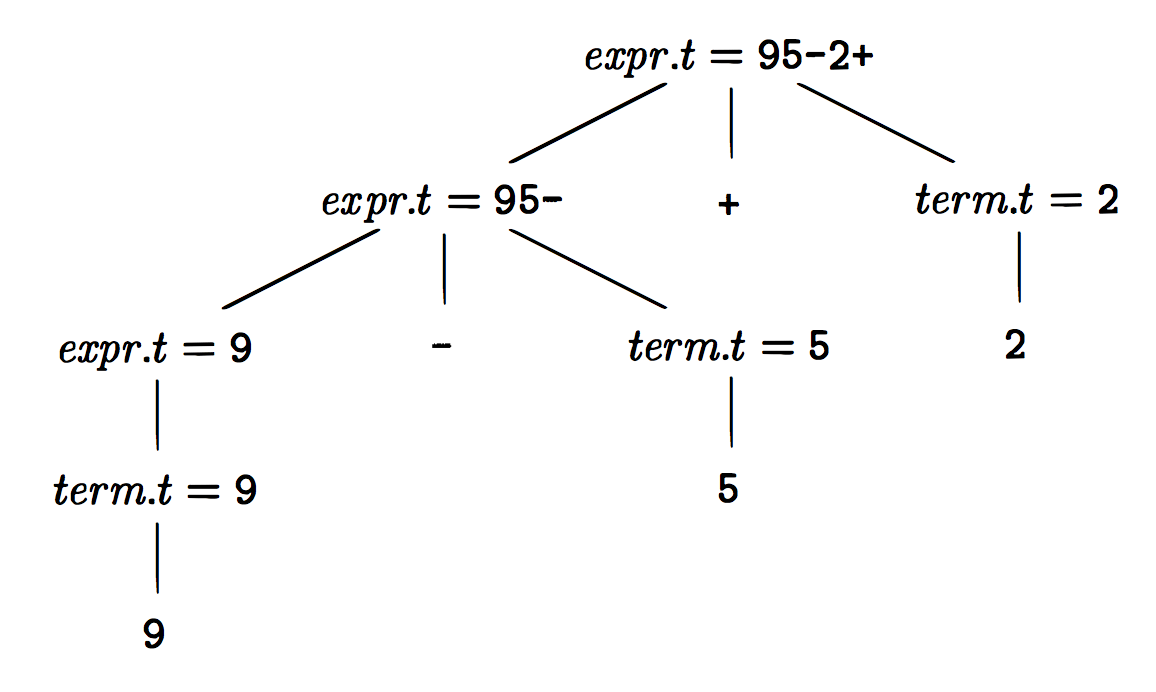
\includegraphics[width=0.7\textwidth]{imgs/syntax_tree.png}
	\caption{Valores de atributos nos nós de uma árvore de sintaxe.}.
	\label{fig:syntax_tree}
\end{figure}

\subsection{Geração de Código Intermediário}

As classes indispensáveis para geração do código intermediário no nosso \textit{front end} se encontram no pacote \texttt{inter}. Neste pacote implementamos a hierarquia da classe \textbf{Node}.

Os dois descendentes diretos de \textbf{Node} são:
\begin{itemize}
	\item \textbf{classe Expr}: Responsável por nós de expressões. Alguns de seus métodos, juntamente com suas subclasses, geram códigos de desvio para expressões booleanas, tendo o método \textbf{jumping} como essencial nessa tarefa, pois é ele quem vai declarar o desvio propriamente dito. Expressões lógicas e aritméticas são exemplos de construções possíveis com \textbf{Expr} e suas subclasses.
    \item \textbf{classe Stmt}: Responsável por nós de comandos. Os comandos tem a ver principalmente com o fluxo de execução do código, como \textit{loops} \textbf{while}, comandos de decisão, como \textbf{if} e \textbf{else}, e interruptores de fluxo do tipo \textbf{break}. Apesar disso, a operação de atribuição é uma variação de \textbf{Stmt}, tendo sido implementada nas classes \textbf{Set} e \textbf{SetElem}.
\end{itemize}

Chamados durante a execução do analisador sintático(\textbf{parser}), são esses nós que representarão a árvore sintática, apresentada na subseção anterior, a partir da qual é gerado o código intermediário.
